\chapter{\label{chap:chap4}{Interview Results}}

This chapter explore the participants responses to the questions in Table \ref{tbl:questions} by presenting participants' interpretations of the literature-informed quality attributes, taken as result of our pilot study \cite{Refsq_2018}, and their personal evaluation criteria, tied to BDD scenario's characteristics and similar to the author's experience-based criteria \cite{Smart_2014}\cite{Wynne_and_Hellesoy_2012}.

The multiple interpretations of the literature-informed quality attributes had forced us to question if words such as ``concise'' and ``understandable'' would be suited to represent the characteristics of good BDD scenarios. Therefore, we decided to deal with each interpretation of each attribute in separation and threat them all as characteristics. Additionally, the participant's personal evaluation criteria were also treated as characteristics. In Section \ref{chap:chap4_analysis} we group those characteristics into 8 newly-labeled attributes, that we believe are more suited to evaluate BDD scenario's quality than literature quality attributes. Those newly-labeled attributes answer our RQ1 and provide us the insights needed to answer the RQ2 in Chapter \ref{chap:chap5}.

\section{\label{chap:chap4_profile}Participants' Profiles}

\begin{table}[!b]
	\caption{Participants' profiles}
	\label{tbl:profiles}
	\centering
	\begin{tabular}{|m{3cm}|m{3cm}|m{4cm}|m{4cm}|}
		\hline
		\textbf{Participant} & \textbf{Role} & \textbf{BDD experience} & \textbf{Location}\\
		\hline
		P1 & Tester & 3 years & England\\
		\hline
		P2 & Tester & 3 years & Netherlands\\
		\hline
		P3 & Developer & 3 years & Netherlands\\
		\hline
		P4 & Coach & 3 months & Denmark\\
		\hline
		P5 & Tester & 9 months & Netherlands\\
		\hline
		P6 & Tester & 2 months & Netherlands\\
		\hline
		P7 & Tester & 3 years & Netherlands\\
		\hline
		P8 & Dev/Coach & 10 years & Hungary\\
		\hline
		P9 & Coach & 3 years & England\\
		\hline
		P10 & Developer & 6 years & Sweden\\
		\hline
		P11 & Tester & 4 years & Australia\\
		\hline
		P12 & Tester & 3 years & Brazil\\
		\hline
		P13 & Developer & 3 years & Brazil\\
		\hline
		P14 & Tester & 1 year & Brazil\\
		\hline
		P15 & Coach & 5 years & Australia\\
		\hline
		P16 & Developer & 1 year & Brazil\\
		\hline
		P17 & Tester & 4 years & United States\\
		\hline
		P18 & Tester & 4 years & England\\
		\hline
	\end{tabular}
\end{table}

The summary of the 18 participants' profiles can be found in Table \ref{tbl:profiles}. All of them reported being involved with BDD scenarios by writing or reviewing them. The majority of the participants were marked with the ``Test'' role on the table due to their testing background - they worked both on the scenario's Gherkin textual descriptions and on the automation of those steps. The ones marked with the ``Developer'' role worked as developers who used BDD scenarios as inputs for their development tasks. Finally, the ones marked as ``Coaches'' were mainly external consultants who help teams get training on BDD - all of them helped the team reviewing their BDD scenarios Gherkin textual descriptions.

Regarding their location, the majority of participants came from the Netherlands (P2, P3, P5, P6, P7). That majority can be explained by the fact that we had used the Linkedin\footnote{\url{www.linkedin.com}} social network to find people to interview and the Netherlands is the home location of one of the participants -- therefore, intuitively it would make sense to have that social network suggesting people around one's localization. Other participants came from Brazil (P12, P13, P14, and P16), England (P1, P9, and P18), Australia (P11 and P15), the United States (P17) and from other European countries (P4, P8, and P10).

Another common trait is the way participants use BDD scenarios. The majority of them enhance the textual descriptions on BDD scenarios with conversations, be it a prior conversation with different project roles (such as an example mapping session \cite{Wynne_2015}) or a post conversation to validate if the written scenarios made sense to other team members. However, we have also found cases with BDD scenarios being used without conversations. For one participant (P12), BDD scenarios were used only as inputs to their test automation tool. For other two (P13 and P16), BDD scenarios were requirement's documentation, send to the team by the client as upfront documentation made to represent his needs.  

\begin{table}[t]
	\caption{How participants use BDD scenarios}
	\label{tbl:profiles_how}
	\centering
	\begin{tabular}{|m{12cm}|m{4cm}|}
		\hline
		& Participants\\
		\hline
		\textbf{Conversations leads to scenarios} & 1,4,10,11,15,17,18\\
		\hline
		\textbf{Team scenarios are validated by PO} & 2,3,5,6,7,8,9,11,14\\
		\hline
		\textbf{Tester writes test cases into scenarios' format} & 12\\
		\hline 
		\textbf{Scenarios received by the Team as upfront requirements} & 13, 16\\
		\hline
	\end{tabular}
\end{table}

\section{\label{chap:chap4_attributes}Quality Attributes' Interpretation}

Participants' interpretations of each literature-informed quality attribute that could potentially be used with BDD scenarios \cite{Empire_2017} help us understand what words would help to evaluate BDD scenarios. To that end, the answers of Questions 8 and 9 from Table \ref{tbl:questions} were analyzed. Additionally, the answers of Question 10 in the same Table \ref{tbl:questions} helped us to evaluate if something was missing in our list, while the answers of Question 7 (Table \ref{tbl:questions}) helped us to eliminate some attributes, judged as not useful for the participants.

\begin{figure}[h]
	\centering
	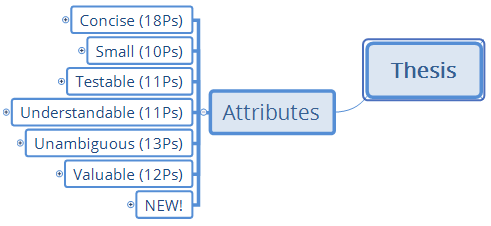
\includegraphics[scale=0.8]{images/overview_attribute}
	\caption{Overview of the attributes to analyze BDD scenarios}
	\label{fig:overview_attribute}
\end{figure}

The results presented in the next sections are based on a partial mind map summarizing the participants' opinions, shown collapsed in Figure \ref{fig:overview_attribute}, that will be break down in each next section topic. Each attribute node contains the number of participants that were able to interpret that attribute presence into BDD scenarios -- for example, all 18 participants were able to interpret concise attribute presence into BDD scenarios, while only 12 were able to interpret the meaning of valuable on that context. Attributes not listed were judged as not useful for BDD scenarios and are discussed into Section \ref{chap:removed}. New attributes, together with their corresponding interpretation, can be found under Section \ref{chap:added}.

%\bigbreak
%\noindent \textbf{( 1 ) Concise}
%\bigbreak
%\bigbreak

\subsection{Concise}

\begin{figure}[t]
	\centering
	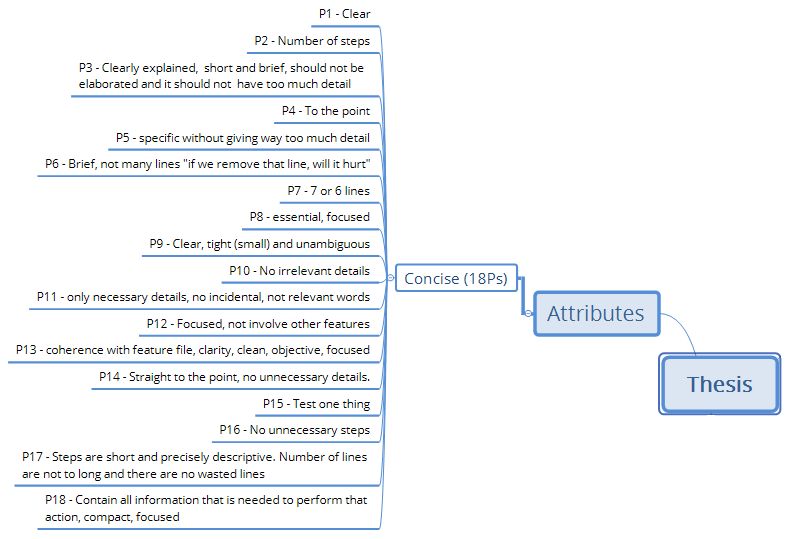
\includegraphics[scale=0.8]{images/concise_attribute}
	\caption{Concise attribute interpretations}
	\label{fig:concise_attribute}
\end{figure}

Concise attribute was deemed important by all 18 participants -- a summary of their interpretation can be found in Figure \ref{fig:concise_attribute}. A concise BDD scenario has no unnecessary details (P3, P5, P8, P10, P11, P16, P17), is focused (P4, P7, P10, P12, P13, P14, P18), clear (P1, P3), and has only a few (P2, P7) brief and comprehensive (P3, P6, P9, P11, P18) steps.

\subsubsection{\textbf{( A ) Not much details}}

% Not much details
P5 reports that a concise scenario \textit{should be specific without giving way too much detail} and should have \textit{no steps longer than they should}. P17 says that \textit{the implication of the word concise is that it's upon the text itself and the length of the scenario, as when you say you have concise steps that means that the steps themselves are short in length and descriptive, and precisely descriptive, right, that are no wasted words and when you talk about a concise scenario that means to me that the number of lines are not to long and again there are no wasted lines, every line has a significant meaning and it says what it needs to say and it's short, sweet to the point fashion}. P9 says it is something clear, tight and unambiguous, while also suggesting to avoid \textit{long step definitions, long steps, things that take a long time to read and understand}. P10 enhances that stating that concise means \textit{a scenario without irrelevant details}, and continues by saying that \textit{some details are important, some should be there, some are important, and if you remove them some things will be scarce anyway. So, if you give me something with lots of details but there's only one or two that is actually important, then you just confuse me} -- and even summarizes his opinion with a metaphor, saying that \textit{there are too many trees, I cannot see the wood}. P8 define scenarios without unnecessary things as essential and P11 define it as \textit{crispy} and refine this stating that \textit{you only have the necessary details on your steps, you do not have incidental words, which are not really relevant to that scenario}. As an example, P11 suggested the use of a data table to isolate data used by many steps and avoiding that same data appearing multiple times on the scenario, as can be seen in Figure \ref{fig:concise_unnecessary_details_parameters_repetition}.

\begin{figure}[t]
	\centering
	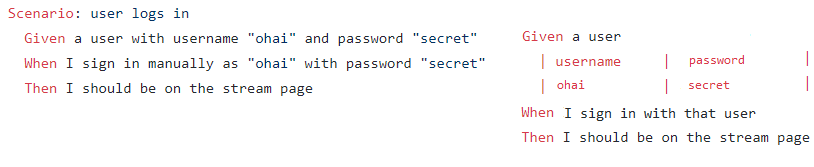
\includegraphics[scale=1.0]{images/logs_in_and_out_feature_parameters_repetitions_not_concise_P11}
	\caption[Scenario with a more concise version]{Scenario from logs-in-and-out feature (left) and its more concise version (right)}
	\label{fig:concise_unnecessary_details_parameters_repetition}
\end{figure}

\subsubsection{\textbf{( B ) Not many steps}}
% Not many steps - P2, P7, P17, P4
P2 said that he \textit{does not like overly long scenarios as the longer they are the most likely they contain implementation details}. P7 also had the same opinion, saying that \textit{a scenario should be small} and that a writer should not \textit{use more than 2 Givens, only 1 When, and then 2 Thens, maybe even 1 because you want to check one thing}. As stated before, P17 is also in favor of few steps - as concise would mean no wasted words and no wasted lines. 

P4 puts steps size under small word, but suggested that steps repetition is something to hurt conciseness. Therefore, to avoid steps repetition on successive scenarios, P4 proposed the use of Background section, as exemplified in Figure \ref{fig:concise_long_background}.

\begin{figure}[h!]
	\centering
	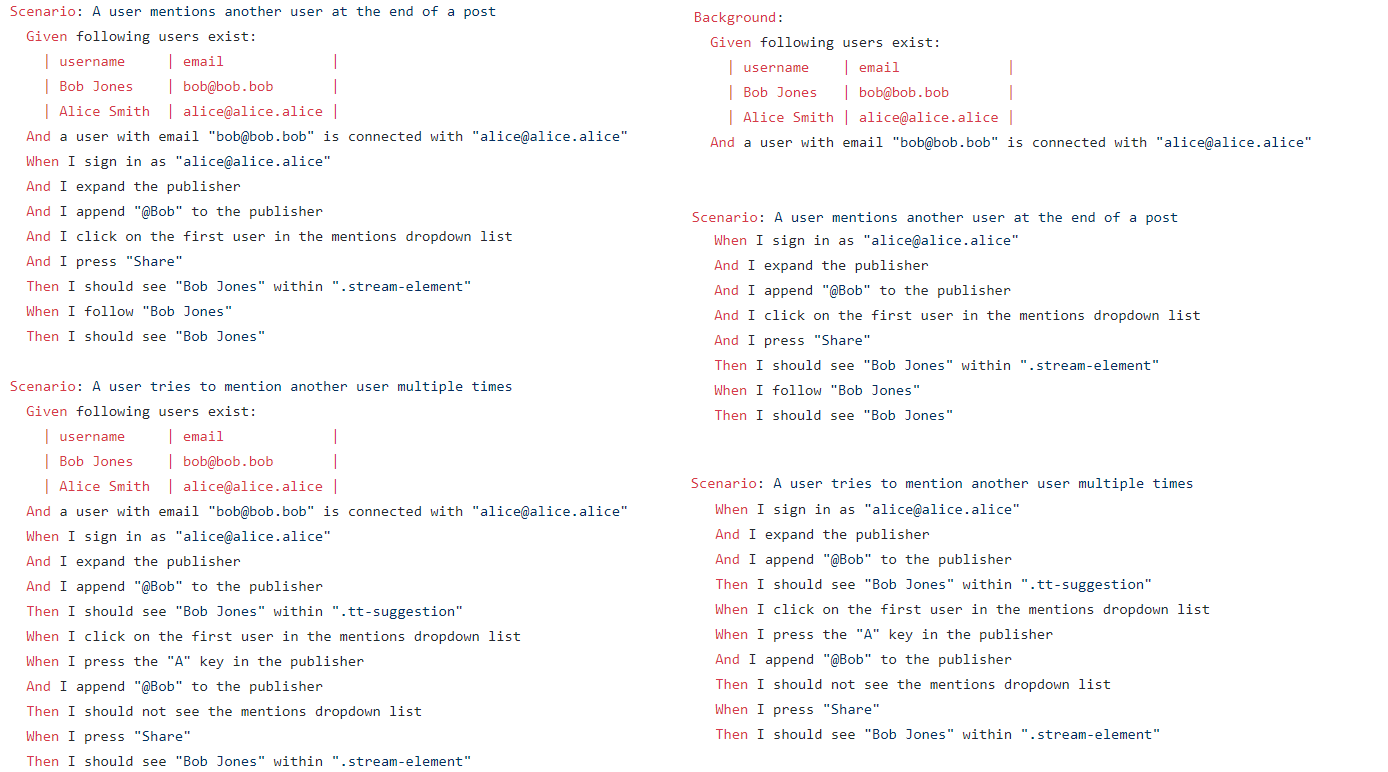
\includegraphics[scale=0.6]{images/mentions_feature_moving_given_to_background_make_it_more_concise_P4}
	\caption[Partial mentions feature and a more concise version]{Partial mentions feature (left) and a more concise version (right)}
	\label{fig:concise_long_background}
\end{figure}

\subsubsection{\textbf{( C ) Focused}}

That check-one-thing opinion enforces P4's opinion that concise is more \textit{to the point}. P12 said it should have a specific focus and should not involve other features. P13 declares that  concise means \textit{clarity, clean, objective, focused}. P14 said it should be \textit{straight to the point, without unnecessary details, one that does not stall, like those who are very long and want to explain many things, it does not need to be very long, trying to explain point-by-point, it can be more direct}. P15 described a scenario on change\_settings feature as not concise \textit{cause it's testing a whole bunch of different things, it's long, it's boring, I do not care} and suggested the change found in Figure \ref{fig:concise_focused_declarative}.

\begin{figure}[t]
	\centering
	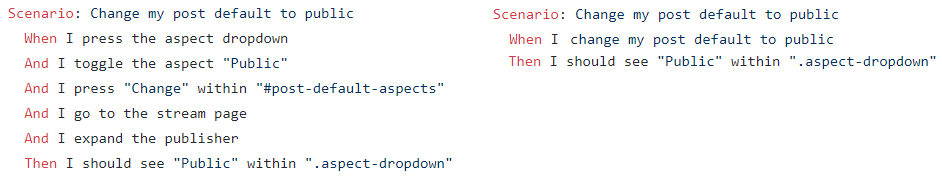
\includegraphics[scale=0.8]{images/change_settings_feature_concise_P15}
	\caption[Scenario's more concise version using declarative language]{Scenario from change settings feature (left) and its more concise version using declarative language (right)}
	\label{fig:concise_focused_declarative}
\end{figure}

\subsubsection{\textbf{( D ) Clear}}
P3's opinions about the steps was that they should be clearly explained, short and brief, should not be elaborated and it should not have too much detail. The word clear also appeared on the report from P1, who said that \textit{you need to write clear steps and you need to be sure that everybody has the same understanding so it's really clear and there's hard to read it differently}.

\subsubsection{\textbf{( E ) Not Unnecessary Lines}}
P6 also referred to it to be \textit{brief and comprehensive} but went ahead and question himself: \textit{if I remove this line, will it actually change the implementation and the outcome? what can I remove without changing the meaning that would make it understandable?} Those questions are somewhat related with P16 opinion that \textit{each step has value, each step is necessary}.

\subsection{Small}

\begin{figure}[t]
	\centering
	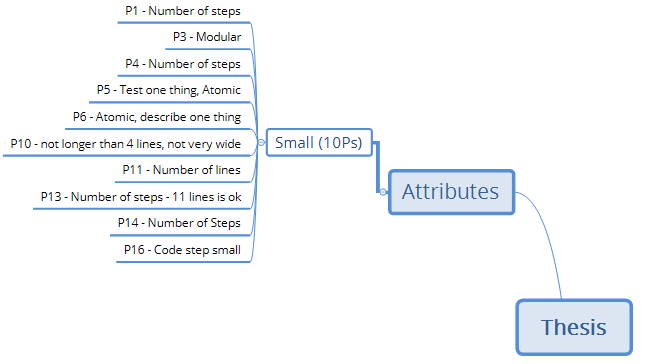
\includegraphics[scale=0.8]{images/small_attribute}
	\caption{Small attribute interpretations}
	\label{fig:small_attribute}
\end{figure}

Small attribute was considered important by only 10 participants -- a summary of their interpretation can be found in Figure \ref{fig:small_attribute}. A small scenario, often considered the same as a concise scenario (P2, P7, P8, P9, P15), is one with just a few steps (P1, P3, P4, P10, P11, P13, P14), which test only one thing (P5, P6) and for which the code to turn it into an executable step is small (P16). Additionally, some participants do not believe that scenarios have to be small (P12, P17, P18).

For P2, P7, P8, P9, and P15, a small BDD scenario is a concise BDD scenario, as both have the same meaning.

\subsubsection{\textbf{( A ) Not Many Steps}}
% Number of steps: P1, P4, P11, P13, P14, P10 (also add length)

The participants P1, P3, P4, P10, P11, P13, and P14 declared that small refers to the number of steps, a problem previously exemplified in Figure \ref{fig:concise_focused_declarative} and in Figure \ref{fig:concise_long_background}. P3 and P10 expand it to also cover the steps length, with P10 saying that \textit{if [the scenario is] longer than 4 lines it's possible not small, if it's wider than the example I looked, some were very very wide, some I would break in some point. If I need a lot of words to express this specific example, it's certainly not small. And if you need lots of lines to do the same thing, it's probably not small} while pointing out to the example in Figure \ref{fig:not_small_due_to_lenghty_line}.

\begin{figure}[t]
	\centering
	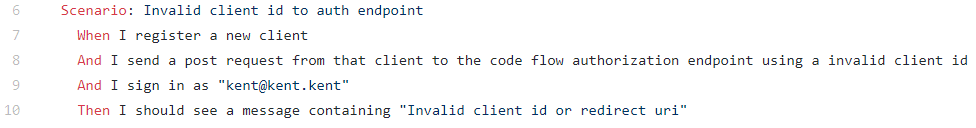
\includegraphics[scale=0.8]{images/oidc_auth_code_flow_small_bad_example_P10}
	\caption{Not a small scenario due to the lengthy line 8}
	\label{fig:not_small_due_to_lenghty_line}
\end{figure}

\subsubsection{\textbf{( B ) Test One Thing}}
% Test one thing - Atomic: P5, P6
Two participants, P5 and P6, reduced the word small to atomic -- the fact that a test describes one thing. P6 provided the example shown in Figure \ref{fig:atomic_small_bad_example}, while also suggesting a more atomic version of it. He described that example as not atomic because \textit{it's testing two things, it's describing two things. These BDD scenarios are obviously written not to describe functionality or be testable -- these are written as test scripts}.

\begin{figure}[t]
	\centering
	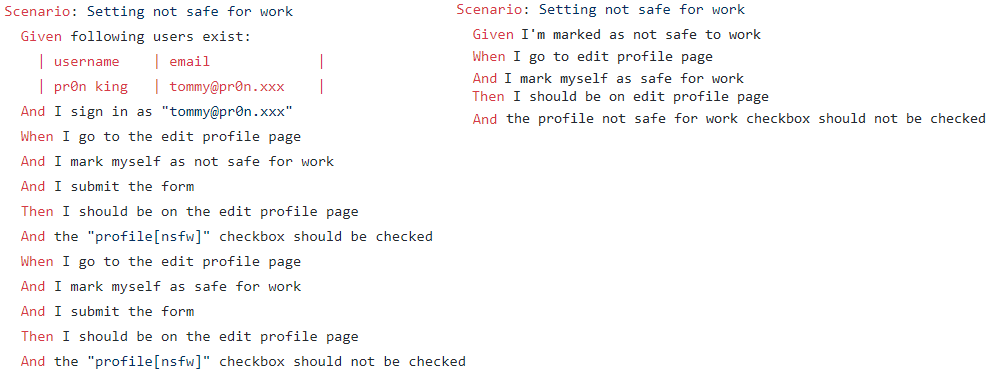
\includegraphics[scale=0.8]{images/not_safe_for_work_atomic_small_bad_example_P6}
	\caption[Scenario that tests two things and a more atomic version]{Scenario that tests two things (left) and a more atomic version of it (right)}
	\label{fig:atomic_small_bad_example}
\end{figure}

\subsubsection{\textbf{( C ) Code Step Small}}
P16 declares that \textit{a scenario cannot be neither small or big, It has to have enough steps, and well described and it's good already}. He sees \textit{small as in the implementation part of that step}.

\subsubsection{\textbf{( D ) Not useful}}

% Not needed
For P12, small is not necessary to evaluate BDD scenarios, as \textit{[a scenario] has to follow the concept of ready, definition of done, of that case. If it's small, nice, but if not it has to be big}. P17 also did not consider small, but for a different reason as \textit{small could refer more broadly to the behavior itself, and that's why I was hesitant to use the word small, because behaviors themselves may not be small behaviors, they may be very big behaviors they may be very complex behaviors}. Finally, P18 also disregarded the small word, as \textit{pretty much on all the agile teams I worked, [small] does not say so much about the requirement but about the deliverable, in other words, we pick up a piece of work that we can manage and not a big piece of work that is risky to do}.

%\bigbreak
%\noindent \textbf{( 3 ) Testable}
%\bigbreak
%\bigbreak
\subsection{Testable}

\begin{figure}[t]
	\centering
	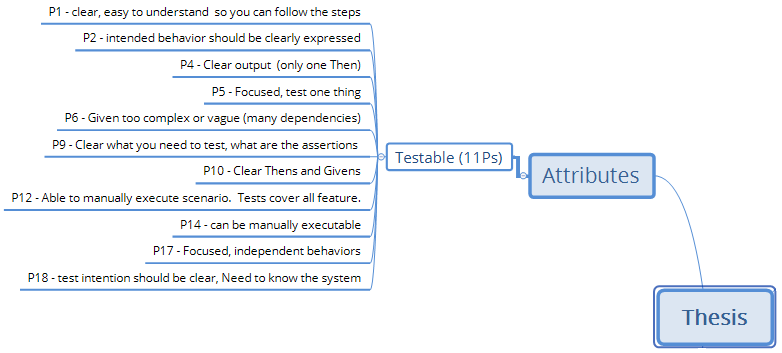
\includegraphics[scale=0.8]{images/testable_attribute}
	\caption[ Testable attribute interpretations]{Testable attribute interpretations}
	\label{fig:testable_attribute}
\end{figure}

Testable attribute was elected important by 11 participants -- a summary of their interpretation can be found in Figure \ref{fig:testable_attribute}. A testable scenario is one who allow the reader to follow its steps (P1, P12, P14, P18), has clear outcomes (P2, P4, P9, P15) and pre-conditions (P6), is independent (P16, P17), focused (P5), and cover all feature (P12), if we analyze all the scenarios together.

\subsubsection{\textbf{( A ) Clear Outcomes and Verifications}}
% Clear outcomes/verifications: P2, P4, P9, P15
For some participants testable means that there are clear outcomes in the scenarios. For P2, testable means that \textit{scenario's intended behavior, or what you are trying to verify, should be clearly expressed in the scenario}. P4 said that a scenario is testable \textit{if it has a clear output, if it has only one Then statement}. P9 also highlighted the need of clear verifications by calling it assertions while stating that a scenario is testable \textit{if it's clear what you need to test, what are the assertions you need to make, it has to be a clear indication of what it is you are asserting}. P15 said that what turns a scenario testable is the fact that \textit{Then step gotta be an outcome you can verify, so the Then step has to be something that can fail}. P18 said that \textit{testable means every time I follow this steps and I'll verify the same behavior}.

\subsubsection{\textbf{( B ) Follow the Steps}}
% Follow the steps: P1, P12, P14, P18
However, for P1, be a testable scenario means \textit{it should be clear, something easy to understand so you can follow the steps}, like the scenario in Figure \ref{fig:testable_as_can_follow_steps}. That same idea is explored by P12 and P14, who said that it is important to be able to manually execute the scenarios. P18 also said that \textit{testable means every time I follow this steps and I'll verify the same behavior -- that every time I follow, I setup this scenario and know I'll get the same results}, and concluded by saying that he \textit{would need to know what the system is actually capable of doing}.

\begin{figure}[t]
	\centering
	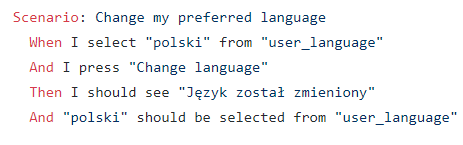
\includegraphics[scale=0.8]{images/change_settings_feature_testable_example_P1}
	\caption[\hspace{2mm}Testable scenario due to the ability to follow the steps]{Testable scenario due to the ability to follow the steps}
	\label{fig:testable_as_can_follow_steps}
\end{figure}

\subsubsection{\textbf{( C ) Clear and Simple Givens}}
% Clear/simple Givens: P6
P6 stated that testable attribute is reflected on the Given steps, as \textit{if your Given conditions are overly complex or very vague then stuff becomes hard to test, that's mostly because the setup for a test is overly complex. And if the setup is overly complex than it means your software architecture is overly complex.}

\subsubsection{\textbf{( D ) Focused}}
% Test one thing, focused: P5
The focused adjective, already mentioned in the concise attribute section and exemplified in Figure \ref{fig:concise_focused_declarative} was also associated to testable attribute. For P5, \textit{the Given/When/Then [structure] helps, to give you focus, to test one thing. And also, not go Given, When, Then, When, Then, When, Then. Because then you are writing a novel, not a scenario. Given this and this, And this, And this, And this...then maybe you are doing something that is not easily testable because it have too many pre-conditions. So we would say Given this and this, And And And And And, When, And And And And, Then, And And And. What are we testing now? Or maybe we are trying to do too much at once?}.

\subsubsection{\textbf{( E ) Independent}}
% Independent: P16, P17
Independence of behaviors was also associated with testable attribute. P16 said that a testable scenario should be \textit{as auto-sufficient as it can} in order to achieve independence of scenarios. P17, when asked what attribute would be impacted if one scenario depend on another, answered: \textit{testable, because if you have interdependent scenarios, that means the problem on one scenario might affect the other. So run one scenario and that should be ok, run it right after the other and it may ruin everything. So, absolutely testable}. 

\subsubsection{\textbf{( F ) Completeness}}
% Scenarios cover all feature: P12
Additionally, for P12, testable represents how complete the scenarios' coverage of the feature behavior is, saying that \textit{if it's not testable I can't even measure the test's coverage}. 

\subsubsection{\textbf{( G ) Not useful}}
% NO, cannot see it on scenarios, it's a product's characteristic: P3, P7, P8, P10, P11, P13
Participants P3, P7, P8, P10, P11 and P13 said that testable is not related with scenarios, but with the product or system being tested.

%\bigbreak
%\noindent \textbf{( 4 ) Understandable}
%\bigbreak
%\bigbreak
\subsection{Understandable}

\begin{figure}[t]
	\centering
	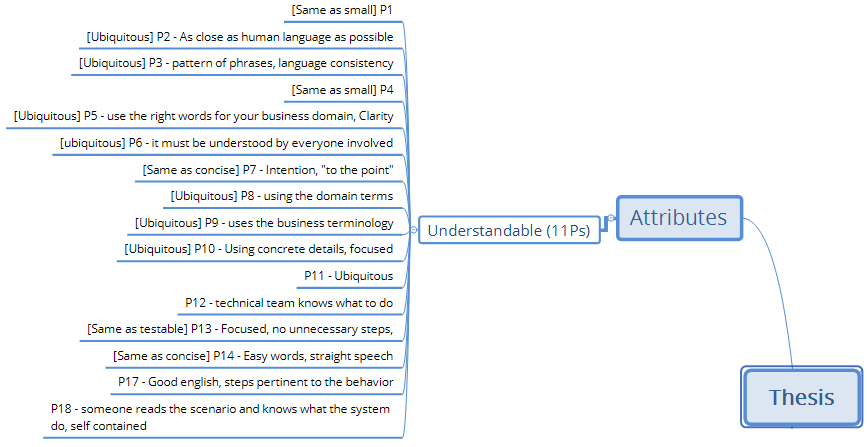
\includegraphics[scale=0.8]{images/understandable_attribute}
	\caption[\hspace{2mm}Understandable attribute interpretations]{Understandable attribute interpretations}
	\label{fig:understandable_attribute}
\end{figure}

Understandable attribute was also deemed important by 11 participants -- a summary of their interpretation can be found in Figure \ref{fig:understandable_attribute}. For some participants, an understandable scenario uses an ubiquitous language (P2, P3, P5, P6, P8, P9, P10, P11, P15), is self-contained (P18), and is written in ``good english'' (P17). For others (P12, P16), understandable means only that technical people understand what to do. The remaining participants (P1, P4, P7, P13, P14) associated understandable as part of other attributes.

\subsubsection{\textbf{( A ) Ubiquitous}}
% Ubiquitous: P8, P9, P10, P11, P15, maybe P2, maybe P6, maybe P5, maybe P18, maybe P3
P11 defined understandable as \textit{quite related to a term we use which is called ubiquitous. What that means is that you basically come up with a terminology which is ubiquitous. What that mean is that all your project team members they are aware of that terminology, and you do not use that terminology where is too technical or business focused alone. It's a terminology that both your technical and business people understand and it is specific to your domain, So, if you do that, all of the scenarios they will be understandable, they will be easy to understand, for everyone, irrespective of their background}. P8 reinforced that idea by saying that \textit{an understandable scenario for me is the one that's using the domain terms}. P9 declared that \textit{it makes sense in terms of the system that is being built}. P10 used the term \textit{concrete details} to refer to the same concept of using business terms on scenarios, by saying that \textit{if you have concrete details you are able to use the same words as business use and turns out you get something that we all understand what you mean and we talk about the same thing}. P15 also suggested the use of an ubiquitous language in the addition of the use of a glossary -- he declared that \textit{the terms in your glossary should be on your scenario}.

For P5, in order to have an understandable scenario a writer have to \textit{make sure to use the right words in your business domain, so people in your domain understand it} -- something also related to ubiquitous term seen before. P5 continued by saying to  \textit{make sure to, on the other hand, not use a particular jargon with HTTP code, that someone may not be familiar with} -- the same advice to avoid technical details and make scenarios more understandable was given by P2. P2 also said that \textit{they [the scenarios] should be as close as human language as possible}. In a similar way, P6 stated that \textit{by understandable you imply that it must be understood by everyone involved. And ahn, when I look at the likes.feature [like the one in Figure \ref{fig:not_understandable_due_to_technical_jargon}], with the CSS elements, that's not understandable by everybody involved}. Finally, P5 compared understandability with clarity by saying that \textit{if you are being too vague, if there's too much room for error, than it would mean something different than I do}. P3 also quoted clarity when saying that \textit{cannot understand [a scenario] for the first few steps} and suggesting the use of a \textit{pattern of phrases} to define language consistency. As all those declarations are related to the consistent use of business language, we also map it to ubiquitous term.

\begin{figure}[t]
	\centering
	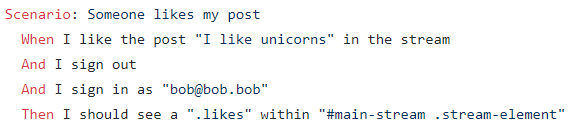
\includegraphics[scale=0.8]{images/likes_feature_understandable_example_P6}
	\caption[\hspace{2mm}Not understandable scenario due to the CSS element]{Not understandable scenario due to the CSS element on Then step}
	\label{fig:not_understandable_due_to_technical_jargon}
\end{figure}

\subsubsection{\textbf{( B ) Self Contained}}
% Self contained, includes all information needed: P18
For P18, an understandable scenario means \textit{is when someone, who has never seen it before, reads the scenario and knows \textit{ok, this is what a user is able to do}, so it is self contained, includes all the information needed}. That fact could be also covered by the ubiquitous terms, but the participant have not make use of that definition.

\subsubsection{\textbf{( C ) Same as Others}}
% Same as others: P1 (small), P3 (valuable), P4 (small), P13 (testable), P7 (concise), P14 (concise)
For P7 and P14, an understandable scenario is straight and \textit{to the point} -- quite similar to their definition of the Concise word. P1 and P4 declared understandable as the same as small. P13 made it the same as testable.

\subsubsection{\textbf{( D ) Good english}}
% Good english (steps tenses, third person): P17, also mentioned by P1
Participant P17 interpreted understandable as in the use of \textit{good english}, the use of \textit{proper grammar, proper tenses, proper point of view}. When referring to tenses, his views are: \textit{the Given steps should either be on past tense or present perfect tense, as it states things you already have; When steps should be active tense because it's something you are doing; Then steps should be present or future tense because that's an outcome that's expected}. The same concern with steps tenses was briefly mentioned by P1, but not associated with any attribute. When referring to the \textit{proper point of view}, P17 referred to the use of \textit{1st person point of view versus 3rd person point of mine, are you saying \textit{I} and \textit{mine} or are you saying \textit{the user} and \textit{the app}}. For P17, \textit{1st person is somewhat ambiguous}.

\subsubsection{\textbf{( E ) Technical People Understand What to Do}}
% Technical people understand what to do: P12, P16
For P12 and P16, understandable scenarios are the ones where technical people understand what to do. For P12, \textit{I read and have no questions on what am I suppose to do. It should have a specific focus, it should take into consideration environment details and business details}, For P16, \textit{it becomes understandable if it's technical, if it has a low granularity on an imperative format with specific steps}.

%\bigbreak
%\noindent \textbf{( 5 ) Unambiguous}
%\bigbreak
%\bigbreak
\subsection{Unambiguous}

\begin{figure}[t]
	\centering
	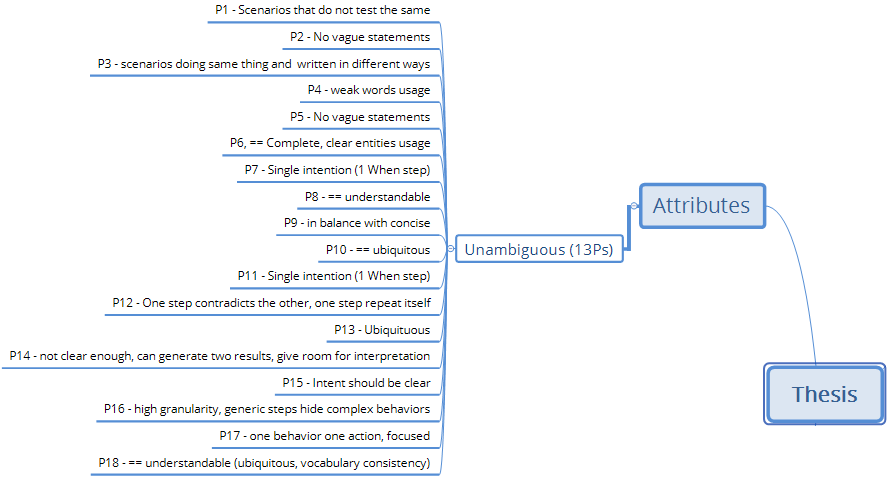
\includegraphics[scale=0.8]{images/unambiguous_attribute}
	\caption[\hspace{2mm}Unambiguous attribute interpretations]{Unambiguous attribute interpretations}
	\label{fig:unambiguous_attribute}
\end{figure}

Unambiguous attribute was reported as relevant by 13 participants -- a summary of their interpretation can be found in Figure \ref{fig:unambiguous_attribute}. Ambiguity on scenarios was interpreted as the use of vague statements, weak words and contradictions (P2, P3, P4, P5, P12, P14), and the lack of a single scenario's intention (P7, P11, P15, P17). Additionally, some concerns were mapped to this attribute, as the fact that scenarios with different descriptions test the same thing (P1, P3), the lack of enough test coverage (P6) and the steps' high granularity (P9, P16).

\subsubsection{\textbf{( A ) Vague Statements}}
% vague/not-clear statements (P2, P5, P14), weak words (P4), contradiction (P12) - P2, P3, P4, P5, P12, P14
One of the sources of ambiguity is bad use of language by using vague, not clear, statements such as \textit{Then the outcome is ok} or \textit{Then the result is good} (both suggested by P2) or \textit{When we see the change in the GUI} (suggested by P4), opening too much room for interpretation (P5, P14). Also, P12 raised the concern of having one step contradicting the other.

\subsubsection{\textbf{( B ) Single Clear Intention}}
% single clear intention (1 When step): P7, P11, P15, P17
Another source of ambiguity is when the scenario intention is not clearly stated - quite often by the use of multiple When steps (P7, P11). P15 was also concerned with imperative steps, where the action was clear enough but the intention was not, like on the one in Figure \ref{fig:concise_focused_declarative}. P17 agreed with that concern and said that an unambiguous scenario is one that has \textit{one behavior, one scenario}.

\subsubsection{\textbf{( C ) Different Scenarios Testing the Same}}
% different scenarios testing same thing - P1, P3
Despite the scenario's description, P1 and P3 reported that different scenarios may be doing the same thing, even if written differently (P3). P1 exemplified it saying that \textit{if you need to test if the connection of the USB on your tablet is working you'd need to be sure the tablet is working, even if the connection is not. So the USB could be broken or the port of the USB could be broken - in the end, you are testing the same thing, because from the testing standpoint of view you are just checking if the tablet will behavior the same if you do not have this USB connection}. 

\subsubsection{\textbf{( D ) Completeness}}
% completeness as part of ambiguous, clear entities usage - P6
For P6, scenario's coverage of the feature should also be mapped into unambiguous attribute, as well as the use of third person rather then first person statements -- referring to \textit{the admin user} rather than \textit{I login as admin user}.

\subsubsection{\textbf{( E ) Ubiquitous}}
% Ubiquitous - P13
P13 declared that unambiguous maps to the ubiquitous term, already mentioned for some other participants as an interpretation for understandable.

\subsubsection{\textbf{( F ) High Granularity}}
% High granularity (steps hide complexity): P9, P16
The participant P16 declared the use of steps written with a declarative language as another source of ambiguity due to the fact that it can hide a lot of implementation details. P9 described the same concern as P16, saying that understandable should be in balance with concise \textit{because the less ambiguous they are, the more complicated they might need to look}.

\subsubsection{\textbf{( G ) Same as Others}}
% Same as others: P8 (understandable, ubiquitous), P9 (concise, in balance), P10 (understandable, ubiquitous), P18 (understandable, ubiquitous)
For the other participants (P8, P9, and P10) unambiguous attribute should be the same as understandable due to the fact that the ubiquitous term covers both attributes. 

%\bigbreak
%\noindent \textbf{( 6 ) Valuable}
%\bigbreak
%\bigbreak
\subsection{Valuable}

\begin{figure}[t]
	\centering
	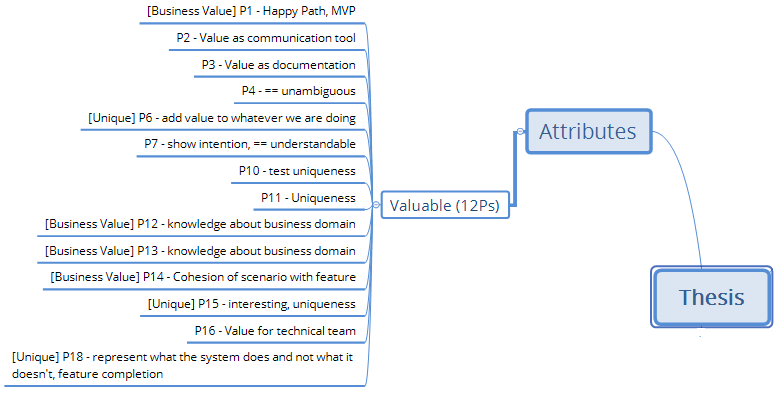
\includegraphics[scale=0.8]{images/valuable_attribute}
	\caption[\hspace{2mm}Valuable attribute interpretations]{Valuable attribute interpretations}
	\label{fig:valuable_attribute}
\end{figure}

Valuable attribute was considered important by 12 participants -- a summary of their interpretation can be found in Figure \ref{fig:valuable_attribute}. A valuable scenario is unique (P6, P10, P11, P15, P18) by validating some different and interesting behavior. Some participants could not identify how valuable a scenario is by reading their scenario description alone -- that characteristic would have been discussed with other team members during formal or informal conversations (P5, P8, P9, P17). Some participants preferred to say a scenario should have value for the business (P1, P12, P13, P14), to the technical team (P16), as a documentation source (P3), or as a communication tool (P2). 

\subsubsection{\textbf{( A ) Unique}}
% Unique - P6, P10, P11 (+ business value), P15, maybe P16, P18 (+ Complete)
For P6, \textit{valuable makes sense because you have to think of a scenario - is this scenario going to add value to whatever we are doing?}. P10 exemplified it further by saying that a scenario is \textit{valuable if we are talking about something that is not covered previously. It's not valuable if we verify that we can do the same thing multiple times. We can search for different books, different titles, we can buy them if we are talking about an e-commerce site, but it's not so valuable to verify that we can buy multiple different titles, it's enough to verify if we can buy one or maybe two, but do the same thing again does not bring us value, it's just more of the same}. For P15, value \textit{is interesting -- is it testing something fundamentally different to the other scenarios}. P18 defined valuable by saying that scenarios \textit{should not be repetitive, if you are having multiple scenarios and they are testing the same behavior, they are redundant -- it's valuable if you have one, that cover it, and that's it}. Finally, P16 declared that \textit{[scenarios] should have a certain importance on their own}, indicating something similar to uniqueness as well.

\subsubsection{\textbf{( B ) Business Value}}
% Business value only: P1 (Happy Path, MVP), P12, P13, P14
P11 agreed that uniqueness should belong to valuable, but that attribute should also cover the importance of a scenario for business people. P1 said that her team \textit{create the scenarios that has more value for the implementation part - like the happy path of a feature, as we need to be sure it's there as this is what is expected to work because this is our main deliverable}. Both P12 and P13 decided how valuable a scenario is by their knowledge about their business domain. P14 decided what are the important scenarios for the feature by the fact it employs important actors or \textit{buying} customers -- also based on his business knowledge and the value to the business.

\subsubsection{\textbf{( C ) Covered on Conversations}}
% NO - Covered on conversations: P5, P8, P9, P17
For P8, valuable comes from discussions with the team, as they \textit{only makes scenarios for things that are valuable}. For P9, valuable has \textit{more to do with Scrum and Agile rather then BDD scenarios}. P5 defined it as \textit{what is worthy testing and what's not worthy testing}, and continued by saying that \textit{I might think that hey, this could go wrong, is that something that should be tested and either yeah, it could go wrong and the probability is low so never mind or that could never happen for technical reasons, so never mind}. For P17, \textit{the value of the scenario is really on the value of the behavior, how important is this behavior for my team, how important is this behavior for the feature}.

\subsubsection{\textbf{( D ) Other values}}
% NO - P2 (Value as Communication), P3 (Value as Documentation), P16 (Value for Technical Team)
Some other meanings of valuable appeared: for P2, those scenarios are a communication tool, so the communication and acting up on the misunderstandings that's what's valuable; for P3, \textit{what value it brings to me is the documentation}. Those opinions did not tied how valuable a scenario is to their scenario description, and therefore could not be used to evaluate a scenario's quality. 

For P16, the scenarios should have value to the technical team alone by being described in a low details' granularity. 

\subsubsection{\textbf{( E ) Same as Others}}
% Same as others: P4 (Unambiguous), P7 (Understandable)
P7 said business value is represented by showing the scenario intention, thus being understandable. For P4, \textit{the value part would be unambiguous to me without additional elaboration on what's a valuable scenario description}.

%\bigbreak
%\noindent \textbf{( 7 ) Removed Attributes}
%\bigbreak
%\bigbreak

\subsection{\label{chap:removed}Removed Attributes}

Prioritized, Negotiable, Feasible, and Estimable were largely regarded as not useful to evaluate BDD scenarios textual descriptions, as either they are useful only for conversations around scenarios, suited for feature file (sets of scenarios) only, dependent on steps' technical implementation knowledge, or are project's domain knowledge -- as summarized in Table \ref{tbl:attributes_removed}.

\begin{table}[t]
	\caption{Summary of removed attributes}
	\label{tbl:attributes_removed}
	\centering
	\begin{tabular}{|m{4cm}|m{2.5cm}|m{2.5cm}|m{2.5cm}|m{2.5cm}|}
		\hline
		\textbf{Reason} & \textbf{Estimable} & \textbf{Negotiable} & \textbf{Feasible} & \textbf{Prioritized}\\
		\hline
		Technical knowledge & P1, P5, P6, P10, P18 &  & P1, P6, P8, P10, P17 & P8\\
		\hline
		Domain knowledge & P3, P12, P13 & P12 & P3, P12, P13, P16 & P8, P12, P14\\
		\hline
		Conversations & P11, P15 & P5, P7, P11, P15, P17 & P3, P7, P11, P14, P15 & P3, P7, P11, P15\\
		\hline
		Only for Features & P14 & P2, P14 & P2, P15 & P2, P3, P6\\
		\hline
		Not applied at all & P2, P4, P7, P8, P17 & P1, P4, P6, P8, P10, P13, P18 & P4, P5, P18 & P4, P5, P10\\
		\hline
		Other & P16 (granular, imperative) & P16 (PO) & P16 (steps reuse), P17 (feasible to automate) & P1, P3, P14, P17, P16 (PO), P13 (happy path), P18 (Tags)\\
		\hline
	\end{tabular}
\end{table}

P11, who declared those attributes as useful for conversations only, explains his thoughts about those attributes as follows: \textit{So I think the other would already have been considered by the time you reach that stage, because, so if you are remember I was talking about example mapping, which is a step which comes before feature files. So, the way you write your examples, so when you write your examples you need to make sure they are estimable for example. And obviously your scenarios would be derived from examples and therefore will automatically be estimable. So it's more relevant at the time of example mapping rather than feature file}. Similar declarations were heard from all the participants who either have conversations before writing scenarios or validate them after they are written as listed in Table \ref{tbl:profiles_how}.

\subsubsection{\textbf{( A ) Granular and Imperative help on Estimable}}
% granular + imperative help on estimable (P16, ?)
Additionally, some participants (P12 and P16) declared that steps with a low granularity, written in an imperative way and carrying fine grained details, help the technical team to estimate the effort to implement them. P12 have developed a system to aid estimate his work with function points \cite{Pressman_2009} by counting the amount of steps of inputs, outputs, integrations, and so on. P15 agreed with it, but declared that \textit{it may be more estimable all the time, but coming back it loses all the value}. As other participants declared that estimable was not useful for textual scenario quality evaluation, we removed that attribute from our list of potential ones.

\subsubsection{\textbf{( B ) Prioritization}}
% tags helps on prioritization, happy path has the most priority, PO decides priorities alongside the client
Prioritization was another characteristic that was more suited to conversations around features than to analyze textual BDD scenarios. P1 and P16 went as far as saying that the PO defines it, alongside the client. P13 suggested that happy path scenarios may have more priority - a characteristic that P1 had assigned to valuable attribute. P3, P14, P17, and P18 suggested the use of tags to tell a scenario priority, using a scale with ``low'', ``medium'' and ``high'' priority -- a characteristic explored on later sections, which also helps on valuable and understandable attributes. Others (P1, P2, P4, P5, P6, P7, P8, P9, P10, P11, P12, P15, P16) have disregarded prioritization as interesting to evaluate textual scenarios, so we decided to also leave that attribute out of our list. 

\subsubsection{\textbf{( C ) Automation Characteristics}}
% Automation characteristics: steps reuse (P16), feasible to automate (P6?), execution time (P5), flaky tests (?) 
Finally, some comments were more directed to the test automation side of BDD scenarios. P17 is used to review textual scenarios alongside their steps code, so feasibility for him was described by how possible that scenario is to automate -- a characteristic that was deemed unimportant for textual scenarios by others. P5 had show concerns with test execution time, but have not assigned it to any attribute -- therefore, we judge this is not something she would use to evaluate the quality of BDD scenarios. P16 was concerned with the ability to have generic steps, easy to reuse and to create new test cases with different parameters, aligned with his opinion that a valuable scenario is the one more useful for the technical team -- again, not associated only with the textual description of a BDD scenario, our research focus. 

%\bigbreak
%\noindent \textbf{( 8 ) Additional Attributes}
%\bigbreak
%\bigbreak

\subsection{\label{chap:added}Additional Attributes}

\begin{figure}[h]
	\centering
	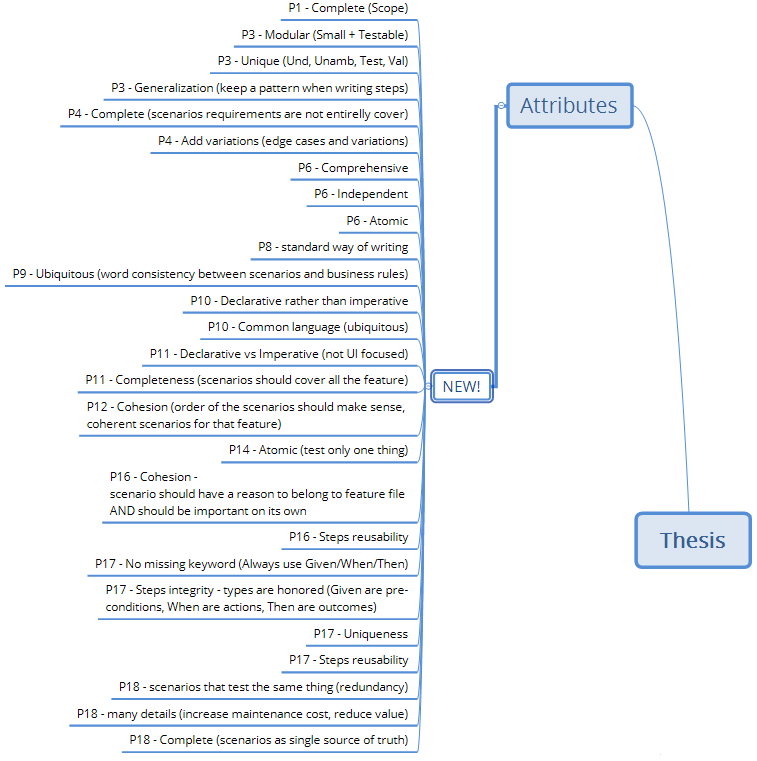
\includegraphics[scale=0.8]{images/new_attribute}
	\caption[\hspace{2mm}New attributes]{New attributes}
	\label{fig:new_attribute}
\end{figure}

Some characteristics outside our list were quoted as important as well, like completeness (P1, P4, P11, P18), coherence (P3, P8), cohesion (P12, P16), integrity (P17), and declarative rather than imperative language (P10, P11, P18). As they were not our investigation focus, not all participants had the chance to provide their opinions about them, so we will just list them here for future reference. Each participant addition is shown in Figure \ref{fig:new_attribute}.

\subsubsection{\textbf{( A ) Complete}}
% Complete: P1 (Scope), P4 (scenarios requirements are not entirely cover, edge cases and variations), P11 (scenarios should cover all the feature), P18 (scenarios as single source of truth)
P1 defined a set of scenarios complete if, during a review, he detects a scenario is missing, what could means the product would be delivered with an unexpected bug. P4 defined it when the scenarios requirements are not entirely covered. P11 suggested that all the scenarios should cover the feature completely -- therefore also adding completeness to the list. Finally, P18 assigned completeness to valuable when considering the feature file as a whole or a set of scenarios. 

\begin{figure}[h]
	\centering
	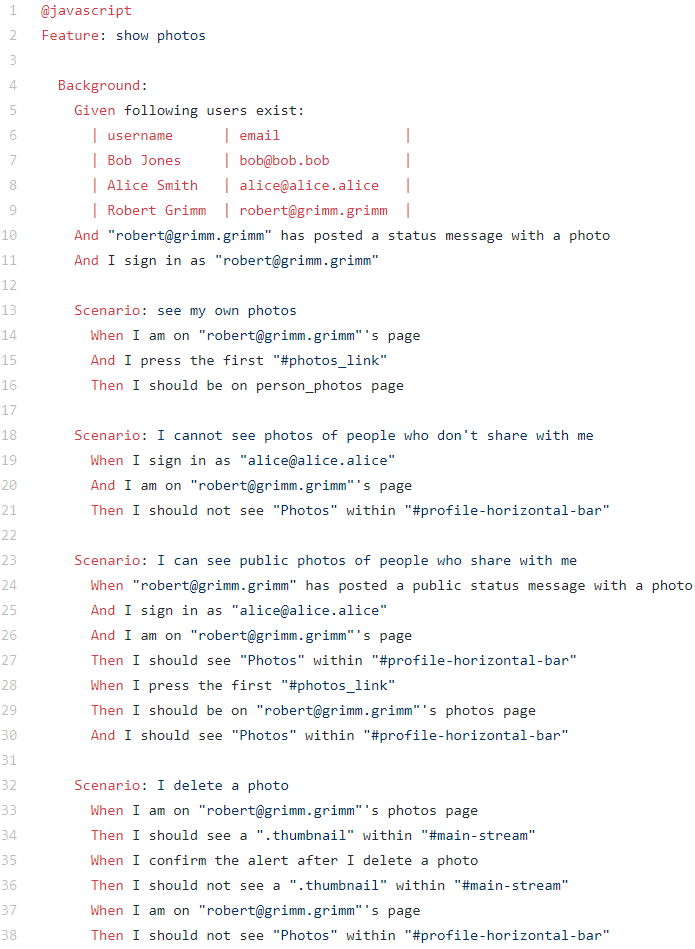
\includegraphics[scale=0.8]{images/complete_profile_photos_feature}
	\caption[\hspace{2mm}Profile photos feature]{Profile photos feature}
	\label{fig:complete_profile_photos_feature}
\end{figure}

On a related way, P4 highlighted the importance of \textit{adding variations} to scenarios, thus having only 1 or 2 scenarios in a feature make it \textit{very thin}. When variations are added, one has to pay attention to missing scenarios as well. When analyzing the scenarios on the profile photos feature file in Figure \ref{fig:complete_profile_photos_feature}, P4 declared it to \textit{raises more questions or concerns}, as \textit{there is no thing in this feature if Robert deletes a profile photo, so can Alice continue to see it? That is not really described, so that would raise a concern on me, something that says the feature is not complete}.

\subsubsection{\textbf{( B ) Writing Patterns}}
% Generalization/Coherence: P3 (Semantics, keep a pattern when writing steps), P8 (standard way of writing)
Coherence was referred to P3 when talking about how his team \textit{define the semantics on how you write the scenario [...] you follow the same pattern even if you have a different application}. According to him, \textit{you can have 3 or 4 business annalists working in the same application, if it's really big, and everyone can come with their own way of explaining a scenario -- so if you define a semantic like, first it should be, you know, the user or the something, the user or the entity for example and then it should be followed by a word then the context. These kinds of semantics really helps everyone to follow the same pattern. Or at least they would be written in similar pattern}. P8 referred to it as \textit{consensus about the scenarios}, when stating that \textit{BDD projects should be under consensus so if they are using this way then it should be used always that way within the same project}. Therefore, coherence, or keeping the same standard way of writing, is another word that could be used to evaluate sets of scenarios.

\subsubsection{\textbf{( C ) Cohesion}}
% Cohesion: P12 (order of the scenarios should make sense, coherent scenarios for that feature), P16 (scenario should have a reason to belong to feature file AND should be important on its own)
Within the context of component-level design for object-oriented systems, cohesion implies that a component or class encapsulates only attributes and operations that are closely related to one another and to the class or component itself \cite{Pressman_2009}. Within the context of BDD scenarios, P16 said that \textit{scenarios should have a reason to belong to a given feature file} and P12, while also agreeing, added that the order the scenarios are presented on a feature file should make sense.

\subsubsection{\textbf{( D ) Integrity}}
% No missing keyword, steps integrity: P17
P17 highlighted the importance of using the three BDD keywords, Given/When/Then, in all the scenarios, while also keeping the integrity of their usage. He declared that \textit{have sometimes seen people do, to try to circumvent the rule of strict steps ordering, is they will start turning Then verifications into When steps, they will say something like \textit{When I'm on Alice's page, And I should see look at this dog, Then I focusing And ...} - they are violating the integrity of the steps type, and that's no more behavior driven than the original procedure}. 

\subsubsection{\textbf{( E ) Declarative rather than Imperative}}
% Declarative rather Imperative: P10, P11, P18
Additionally, some participants (P10, P11, P18) highlighted the need to enforce the use of declarative language, as seen in Figure \ref{fig:concise_focused_declarative}, by turning it into an attribute on its own, in separation of concise. P10 said that \textit{you can think about one thing, and that can be done in two different ways, could be both declarative and imperative}, as his interpretation of conciseness focus only on the lack of unnecessary details. P11 also had the same focus and thus put the use of declarative language in separation of every other attribute. P18 interpretation for conciseness, to have \textit{crispy, very clear} scenarios, also have not had room for the use of declarative language and therefore that characteristic was kept in separation as well.

\subsubsection{\textbf{( E ) Same as Others}}
% Already covered: Unique (Valuable, P3, P17), Atomic (Small, P6, P14, P18), Reusability (P16, P17), Ubiquitous (Understandable, P9, P10), Independence (Testable, P6), Modular (Testable, P3)
Finally, some participants have suggested to transform into additional attributes some characteristics assigned by other participants, like: uniqueness (P3, P17), already covered under valuable attribute; atomic (P6, P14, P18), already covered under the small attribute; steps re-usability, a characteristic out of our scope due to the focus on the scenario's test automation side; ubiquitous (P9, P10), already covered under understandable; independence (P6), already covered under testable attribute; and modularity (P3), already covered under the testable attribute section.

\section{\label{chap:chap4_criteria}Participant's Criteria}

In order to better understand how each attribute presence or absence is reflected on a BDD scenarios, participant's criteria, more tied to the actual textual scenario than generic attributes and similar to author's experience-based criteria \cite{Smart_2014}\cite{Wynne_and_Hellesoy_2012}, were taken from the answers of Questions 5 and 6 in Table \ref{tbl:questions}. Additionally, those criteria were tied back to the attributes in Question 13 (Table \ref{tbl:questions}), in the hope it would refine our literature-informed quality attributes and enhance them with good and bad practices -- a refinement that have not be possible due to the multiple interpretations of the literature-based quality attributes.

\begin{figure}[h]
	\centering
	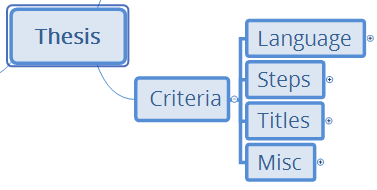
\includegraphics[scale=0.8]{images/overview_criteria}
	\caption[\hspace{2mm}Overview of the criteria to analyze BDD scenarios]{Overview of the criteria to analyze BDD scenarios}
	\label{fig:overview_criteria}
\end{figure}

The results presented in the next sections are also based on a partial mind map summarizing the participants opinions, shown collapsed in Figure \ref{fig:overview_criteria}. This summary will be expanded in each section, on which several criteria are grouped together into four groups: language criteria, steps criteria, title criteria, and others criteria. 

%\bigbreak
%\noindent \textbf{( A ) Language}
%\bigbreak
%\bigbreak
\subsection{Language}

\begin{figure}[t]
	\centering
	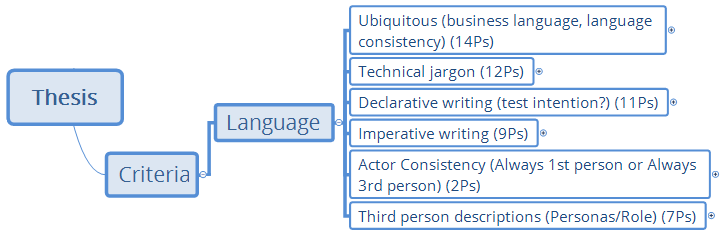
\includegraphics[scale=0.8]{images/language_criteria}
	\caption[\hspace{2mm}Language criteria to analyze BDD scenarios]{Language criteria to analyze BDD scenarios}
	\label{fig:language_criteria}
\end{figure}

Language groups together characteristics, summarized in Figure \ref{fig:language_criteria}, that depend on writing decisions, such as the use of business terms instead of technical ones, the declaration of actions rather than the description of steps and the subject point of view.

\subsubsection{\textbf{( A ) Ubiquitous}}
%Consistent use of Business Language (Ubiquitous)
The consistent use of business language, like \textit{a glossary that appears consistently on all scenarios} (P9) is regarded mostly as a good practice. P9 also referenced it properly, saying that \textit{in domain driven design that is known as ubiquitous language} -- the same term that we mapped as one of the meaning of understandable attribute in a previous section. 

Participants have mapped it as a good practice impacting understandable (P1, P2, P3, P5, P6, P7, P8, P9, P10, P11, P15, P18), unambiguous (P3, P8, P10, P13), and concise (P4, P11) attributes and as a pain-point for the estimable (P3) attribute -- for P3, \textit{if it's on technical language it's very easy to estimate}.

\subsubsection{\textbf{( B ) Technical Jargon}}
%Technical jargon
In opposition, the use of technical language, or technical jargon, as expressed in Figure \ref{fig:not_understandable_due_to_technical_jargon}, is considered as harmful for understandable (P1, P2, P5, P6, P8, P9, P11, P14, P17, P18), concise (P2, P10), unambiguous (P2), small (P10), valuable (P7), and testable (P10) attributes. Other examples of technical language would be the use of HTTP response codes (P5), or automation steps on the UI like \textit{When I click a button}.

\subsubsection{\textbf{( C ) Actor Consistency}}
%Personas/Roles/3rd person, consistency
Despite the consistent use of business language terms, some participants also pointed out the need to write steps using third person point of view. P18 highlighted the use of third person as a good thing as \textit{it could get your whole team to think like the user and that would be very useful}. P18 continued by saying that \textit{``I'', as in ``I reading it'',  or ``I the QA'' or ``I the developer'', what I do might be a bit different of what the actually would be doing. It helps to set a mindset, when you are thinking more about the user}.

A way to use third person point if view is to build personas -- fictional characters that are meant to represent the different types of people who will be using the system, as pointed out by Smart \cite{Smart_2014} on his book about BDD. P2 exemplified this referring how the use of ``alice@alice.alice'', on scenarios such as the one in Figure \ref{fig:concise_focused_declarative} with a step \textit{When I sign in as ``alice@alice.alice''}, could be changed to \textit{Given I sign in as Alice}. He explained that decision saying that \textit{you have a object, a persona, called Alice, with a number of properties, one of them being her email address, and you have that, so you do not have to specifically define those variables again}.

Another way to use third person point of view is to describe roles of users, as described by P6: \textit{but if you say ``an user must be logged in'' that's already a bad line because the user can have a variety of meaning, it can be, it can have administrator or a guest user or, no, the user must be logged in so it cannot be a guest user. It can be an user with access rights type A or type B or anything like that. What you should say is ``an user in group XYZ'' or ``the user with template ABC'' and then you have a bunch of users template where you define what your actual setup is}.

The use of all forms of third person point of view is considered as a good practice and enhances the understandable (P2, P7, P17), concise (P9), unambiguous (P6), and valuable (P14, P18) attributes. Additionally, some participants (P16, P17), while inclined to use third person point of view on their steps, were already happy only with consistency - using always first person or always third person.

\subsubsection{\textbf{( D ) Declarative rather than Imperative}}
%Declarative/Imperative writing
Despite the language terms and the point of view, there is also the concern about how granular a scenario step description should be, as exemplified in Figure \ref{fig:concise_focused_declarative}.

P2 said scenarios should \textit{focus on the problem, not the solution} and P8 called it as \textit{declarative}, with \textit{imperative} being his opposite. For P17, \textit{Gherkin is meant to be declarative because it tries to describe behavior that add business value, it's not necessarily to give the implementation on how that behavior works}.

P17 explained that difference in the writer mindset, saying that \textit{the difference between declarative and imperative is in how granular your details are in your steps}. He also said that \textit{the declarative way to say something would be ``Given the user is logged into the app'', very simple, very descriptive, it's not necessarily saying how is done, it's saying what is done}. 

P5 warned about how imperative writing may impact the maintainability of scenario, saying that \textit{if you write it like this [in imperative form] and the UI changes than this test will break. Whereas if you write it further, ``I block the user so and so'', the change you have to make is much smaller, because it's at a lower level, somewhere in the supporting code}.

In opposition, P17 also described the imperative way of writing this action as \textit{Given the user enters www.whatevermywebsiteis.com And the user enters the username field And the user enters andrewknight And the user enters the password field And the user answers abc123 When the user clicks the login button Then the page is rendered}. For P17,  \textit{ultimately, for the automation sake, those specific actions would need to be taken, because you need to use something like Selenium web driver to click various elements on the page, but the thing is, that's impertinent at the Gherkin level right, Gherkin is meant to be descriptive, it's meant to be high level, it's meant to be business oriented, it's meant to be behaviors and not necessarily neat gritty little steps}. 

For those participants who mix scenario's writing with conversations, either before or after the writing of them, the use of declarative language is seen as a good practice that enhances understandable (P7, P8, P9, P14, P15), testable (P1, P2, P5), concise (P8, P17), and unambiguous (P14, P15) attributes. Imperative language usage was considered as harmful for testable (P1, P18), small (P5), understandable (P7), and concise (P17). 

However, P12 and P16, who use scenarios with a technical approach in mind, considered declarative form of writing harmful for understandable (P12, P16), estimable (P16), feasible (P16), testable (P16), unambiguous (P16), and valuable (P16) attributes. Imperative writing was considered a good practice that enhances estimable (P12, P16), understandable (P12, P16) feasible (P16), testable (P13, P16), unambiguous (P16), and valuable (P16) attributes.

%\bigbreak
%\noindent \textbf{( B ) Steps}
%\bigbreak
%\bigbreak

\subsection{Steps}

Steps characteristics, summarized in Figure \ref{fig:steps_criteria}, look at how many steps a scenario have, how long are they, and what step keyword to use.


\subsubsection{\textbf{( A ) Few and Short Steps}}

% Few and short steps
Having long scenarios with many steps, as shown in Figure \ref{fig:concise_focused_declarative}, is considered harmful mainly for concise (P2, P3, P6, P7, P8, P9, P15, P17, P18) and small (P1, P3, P4, P5, P10, P11, P13, P14), as already discussed on those attributes' sections. There were also reports about it affecting unambiguous (P3), understandable (P14), and testable (P18) attributes. In a similar way, lengthy statements, as shown in Figure \ref{fig:not_small_due_to_lenghty_line}, are considered harmful for concise (P3, P5, P7, P9, P17), small (P1, P3, P4, P10), and understandable (P17) attributes.

P17 said that, \textit{the more imperative you write your scenarios the more lines it will have, so if you have too many lines, you can kinda guess, you can probably state some of those things a little bit better}, which could indicate that having fewer steps is not a proper goal, but having scenarios written in a declarative format rather than imperative would. 

\begin{figure}[t]
	\centering
	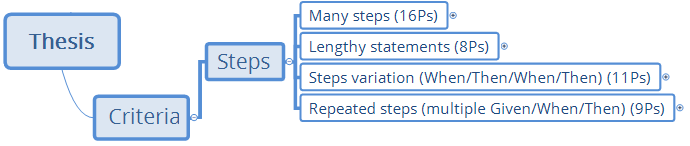
\includegraphics[scale=0.8]{images/steps_criteria}
	\caption[\hspace{2mm}Steps criteria to analyze BDD scenarios]{Steps criteria to analyze BDD scenarios}
	\label{fig:steps_criteria}
\end{figure}


\subsubsection{\textbf{( B ) Steps Order}}
% Steps order
Additionally, there was a concern with the natural step order of Given/When/Then being violated. On examples such as in Figure \ref{fig:steps_order_alternating_when_then}, from which P17 commented as a \textit{major BDD violation}, which he explain saying that \textit{one of the hard and fast rules that I apply for writing BDD scenarios is the strict ordering of steps, Given/When/Then order}. P2 said that alternating the use of When and Then words \textit{means that you need to split up in two smaller scenarios} and that \textit{a good test is exactly one verification and alternating when and then means you are testing more than one thing in the same scenario}. P6 described it as \textit{expanding your scenario to cover multiple pieces of functionality}, and added that \textit{I do not like chaining in scenarios because you are not considering those scenarios might take future changes. Because if you build your scenarios like this, then how can you build code that only does one thing - you get bad code as well, as a result of bad scenarios}.

\begin{figure}[t]
	\centering
	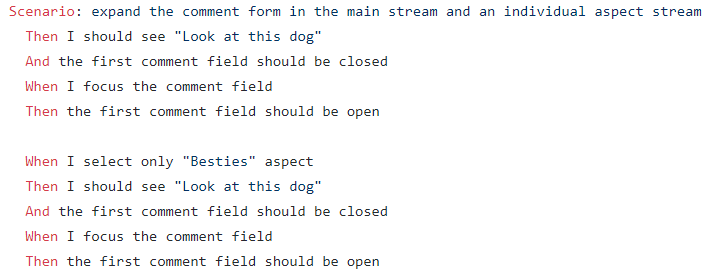
\includegraphics[scale=0.8]{images/comments_feature_steps_order_P17}
	\caption[\hspace{2mm}Scenario alternating When/Then steps]{Scenario alternating When/Then steps}
	\label{fig:steps_order_alternating_when_then}
\end{figure}

Therefore, this violation of the natural step order is considered a bad practice that affects understandable (P2, P4, P8, P10, P14, P17, P18), concise (P2, P3, P8, P9, P14, P18), testable (P2, P7, P18), unambiguous (P3, P14, P17), valuable (P3, P18), and small (P6) attributes. 

\subsubsection{\textbf{( C ) Steps Repetition}}
% Steps repetition
In a similar way, the multiple repetition of the same step, demonstrated by the excessive use of Given/When/Then steps in sequence or the ``And'' keyword, is also judged a bad practice. P4 summarized it saying that \textit{If there are many Ands than it makes it probably harder to understand}. Additionally, P6 declared that multiple repeated steps, like the example in Figure \ref{fig:atomic_small_bad_example} may indicate those scenarios were \textit{written as test scripts} and \textit{not to describe functionality}.

This repetition of the same step bad-practice affects unambiguous (P4, P7, P11, P12, P14), concise (P4, P7, P8, P14), testable (P4, P6, P9), understandable (P4, P7, P14), and small (P5) attributes.

%\bigbreak
%\noindent \textbf{( C ) Titles}
%\bigbreak
%\bigbreak

\subsection{Titles}

\begin{figure}[t]
	\centering
	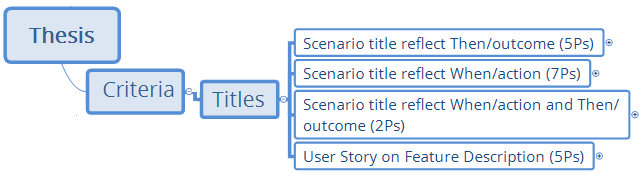
\includegraphics[scale=0.8]{images/title_criteria}
	\caption[\hspace{2mm}Title criteria to analyze BDD scenarios]{Title criteria to analyze BDD scenarios}
	\label{fig:title_criteria}
\end{figure}

Despite analyzing the language and the steps characteristics, participants were also asked to analyze the scenario and feature file titles and descriptions. The characteristics that emerged are summarized in Figure \ref{fig:title_criteria}.

\subsubsection{\textbf{( A ) Feature Description}}
%Feature description
Feature titles and descriptions were often pointed out as \textit{intended business outcome or the indented business value} (P2) in one way or another. That good practice would enhance the understandable (P4, P14) and valuable (P7) attributes.

\begin{figure}[t]
	\centering
	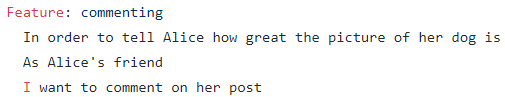
\includegraphics[scale=0.8]{images/feature_description_example}
	\caption[\hspace{2mm}Example of a Feature description on comments.feature]{Example of a Feature description on comments.feature}
	\label{fig:feature_description_example}
\end{figure}

Some participants (P11, P15, P17) have suggested using the user story standard description on feature descriptions. However, P8 did not believe feature descriptions are useful at all, even worse if they have user stories descriptions like in the example in Figure \ref{fig:feature_description_example}. \textit{In this case [comments.feature] this is a user story description which I generally do not like that my feature files to be structured based on user stories because the user stories are somehow arbitrary split of the implementation so it depends on what fits into your Sprint, what is current priority}. And continues saying what he really want to see: \textit{I just want to see right now the behaviour of my application. [...] This feature file is about comments but I do not see any benefit on a user story description like this, so maybe there's lot of other actors that can do comments, so I generally do not put the user story text into the feature files}.

Additionally, some participants (P10, P15) warned about the use of technical details on feature descriptions, such as in the phrase \textit{Access protected resources using auth code flow}, which P15 declared: \textit{I do not really understand what using auth code flow would be. Yeah I can understand \textit{using} and I think I can understand what \textit{auth code flow} might mean but there's probably some less technical that could be used there}.

\subsubsection{\textbf{( B ) Scenario Titles}}
%Scenario titles
Regarding scenarios' titles, participants declared it should either express the intended action (P3, P5, P9, P10, P13, P16, P17) or the intended outcome (P2, P8, P12, P14), or both (P18, P11). Surprisingly, only few have declared it affects an attribute -- from those who did, they mapped it with understandable (P9, P18), testable (P2, P15), and concise (P12) attributes.

%Scenario titles - When/Action
Some participants were concerned with how good the correlation of the scenario title and a When step was. For example, when P9 reads a title that \textit{says it's about a user mentioning another user}, he was \textit{lead to assume that this is the main action, in this example, a user mentioning another user, but the action which would normally be found on the When step, is the ``I sign in as Alice''}. For others, like P10, that also declared it's important to have scenario titles expressing the intended action, \textit{it should not match any step, necessarily, and it should, however, be nice if it tells me what it is doing}.

%Scenario titles - Then/Outcome
For others, the intended outcome is enough, as exemplified by P2, who declared: \textit{I personally like to see a desired outcome scenario name. So regarding the ``Hovercards on the main stream'' scenario, if I split it up for a single scenario for activation and a single scenario for deactivation I'd call the first one ``Hovercards on the main stream can be activated'' and the second one ``Hovercards on the main stream can be deactivated'' [illustrated in Figure \ref{fig:breaking_scenarios_to_allow_better_titles}]. And that's because if you just see scenario names into a reporting tool I'd like to know just with the scenario name and the execution result of that scenario I want to be able to determine what feature in my application works or does not work anymore}. For P15, this intended outcome is \textit{what is I'm sort of testing}, while P8 called it \textit{the goal of a scenario} and, when reading a title phrased as \textit{Comment to the status show page}, he inquired: \textit{what do you want to test here? Are you able to comment? To do a comment? So I would like to have something that describes kind of a business rule, something that says this was fulfilled or not fulfilled, not just a topic}. P17 is pleased without the outcome, as he declared that \textit{many times when you read the action, the outcome is sort of implied}.

\begin{figure}[h]
	\centering
	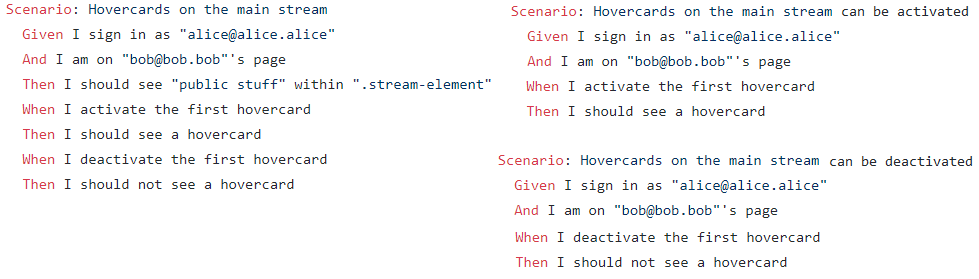
\includegraphics[scale=0.8]{images/breaking_scenarios_to_allow_better_titles}
	\caption[\hspace{2mm}Breaking hovercards scenarios to allow better titles]{Breaking hovercards scenarios to allow better titles}
	\label{fig:breaking_scenarios_to_allow_better_titles}
\end{figure}

%Scenario titles - both
Additionally, there are others who want to see both, outcome and action, expressed on the title -- as P11, who says that a scenario title \textit{should briefly tell me what I'm testing and what I'm expecting as the outcome. So just, obviously if it takes too much space, you would not want to over-complicate things, you would want to keep it brief, otherwise it basically defeats the purpose. So what you could do this, if you would write more text, just add a comment below the scenario keyword. So it would basically appear as informative test, just under scenario keyword, you can do that in a feature file}.

A common goal shared by some participants (P2, P11, P17) was to have scenario titles help on failure reporting. As summarized by P11, if you are able to write good titles, \textit{when this test report is shown to someone, your project manager, your business owner or your tester, they would instantly know, without looking at the steps, what exactly is being validated here, or what would you expected}. P2 added up for that goal by saying that \textit{you are using an living documentation and this is not only for the specification side but also for the reporting side}.

%\bigbreak
%\noindent \textbf{( D ) Additional constructions}
%\bigbreak
%\bigbreak

\subsection{Additional Criteria}

\begin{figure}[t]
	\centering
	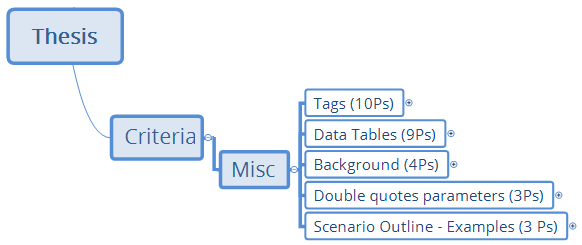
\includegraphics[scale=0.8]{images/misc_criteria}
	\caption[\hspace{2mm}Additional criteria to analyze BDD scenarios]{Additional criteria to analyze BDD scenarios}
	\label{fig:misc_criteria}
\end{figure}

Despite the scenario's language, titles and steps descriptions, Gherkin language allow other types of constructions such as the use of a background section, tags, scenario outlines examples, data tables or double quotes aid to pass parameters. Those characteristics are summarized in Figure \ref{fig:misc_criteria}.

\subsubsection{\textbf{( A ) Background}}
%Background section, only when needed, only with Givens
For P18, a Background \textit{sets the context for the rest of the feature. And when you start reading it, ok, these users will always exist for all these scenarios. So that's useful, but, that's fine, it's also very helpful when you try to automate things, because the Given can be defined to run before each test, so it also helps on that purpose. Actually, one last thing about the Background, potentially it can show, it can be sort of a sanity check to confirm that the entire feature in fact is about one feature so it's tied to one background, so it might help there as well}. However, P15 reflected on the need of a background section, when asking himself: \textit{does adding a Background make it harder for people to read? If it makes it harder for people to read, then no, it's a bad idea. If you've got a quite large number of scenarios, the Background should have a different title as well}. 

P10 said a background section should not mix Given/When/Then steps and \textit{it is most likely the Given stuff}. Additionally, confirming P15's opinion, P10 said that \textit{where we have 3 scenarios in a feature file, I would not put it in the background. It could be argued that this is a duplication [...] but in almost any situation and specially in any test case, I prefer clarity over duplication}.

The use of background section can enhance the concise (P2, P4, P17, P18) and understandable (P2, P4, P17) attributes, as shown before in Figure \ref{fig:concise_long_background}.

\subsubsection{\textbf{( B ) Tags}}
%Tags
Tags were reported as being used for scenario's categorization (P1, P2, P3, P11, P12, P13, P14, P16) and as a communication tool (P3, P7, P10, P15, P17).

%Tags as filters
P1, who has scenarios that run on desktop or mobile, argued that tags can be used to \textit{separate those scenarios}. P11 said \textit{you could have some feature files tagged as end-to-end UI based scenario, some could be tagged as integration, some could be tagged as a component or you could also have feature based tags or module based tags}. P12, P13, P16 also use tags for run specific tests on specific situation 

%Tags as communication tool
Additionally, P15 reported that \textit{tag is all about metadata, so tags are all about adding information from a usage or metadata point of view which is not associated with the behavior}. P1 reported \textit{there are tags for smoke tests -- I have a regression pack which is quite huge and when we need to do a smoke test with just basic scenarios we tag those as smoke}. In the same way, P3 reported \textit{it can give the context of the importance of the scenario or the feature}, and explained it further by saying that \textit{if you categorize your feature and scenarios into mainly different areas, something like UI, or maybe say it depends on integration to start, you know... just a basic story, a back end test, it gives a sense of the importance of this scenario or feature. Where this feature stands from an application stand point of view}. 

%No tags
However, P5 warned about excesses. For P5, \textit{if you are using the tags than you want to be able to run a certain test of sets, given a certain tag, and why would you want to run only a certain set and not all the tests? Because maybe something changed in this area, but if your test suite is fast enough you could run all of them. There would be no need to say in this case I will only need to run there and not those. So this could also be a code smell, excessive use of tags}. Additionally, P2 warned about the use of tags for technical purposes only, when he said that a tag \textit{tells something about the implementation, not about the intention or the behavior of your application and specify something of the intent or the implementation of your test scenarios may not... if you want to group features or scenarios together I think you'd be better of just regrouping the features or placing features into folders, what is more understood by humans than tags that can appear whatever. I do not use those for technical purposes}.

The use of tags affects valuable (P1, P3, P4, P14, P17), understandable (P3, P11), prioritized (P3, P14), and unambiguous (P3) attributes. However, P2 said it can harm understandable due to their technical nature.

\subsubsection{\textbf{( C ) Data Tables}}

Data tables had caused different reactions from participants. As summarized by P8, \textit{tables has pros and cons, such as, well, the pros are for repetitive tests that needs to cover a different range in the input and they could be considered one scenarios. The cons are that you might accidentally bunch many scenarios together that should be kept separate - so it should be less and less easy to read, less clear}.

P11 considered that \textit{tables are a good idea, actually, so instead of having to you know write several lines if you can structure then in a nice table, obviously the table should not have 20 columns, you know, if it's a nice concise small table which is easy to read and as long as it does not have like 20 rows or 20 columns, it looks good, it's easier to read, it's better than writing 10 steps, as it's possible that you are able to summarize them in one table. And that makes much easier to read, as long it is a small, concise table with a minimum at steps, minimum rows and columns}. P14 also agrees with that same opinion of having small tables, and highlights the importance of headers on that table. P18 said \textit{tables are a good way to input data, and that's why most people use Cucumber is because of data tables in particular}. P13 was in favor of even using multiple tables at a same scenario.

However, some participants (P1, P2, P7, P10) would not use data tables at all. For example, P1 said: \textit{I would not use a data table, I'd use examples, because data tables are complex because it's just a bunch of data you can send but you do not really know what's the context in the step. Because you are not setting a variable value, that you have in the middle of the step}. P2 said that, when \textit{creating an end-to-end test using a tool like Selenium}, using tables \textit{is often a sign of bad automated test design if you use tables in those tests, because then basically you are repeating the same process, the same customer flow, with different parameters. And for me that's a sign that those tests with parameters should be executed at the lower level}. P7 dislike data on scenarios, completely. P10 even declared: \textit{I'm not always convinced that they [data tables and examples] lift their own weight. I think it that, if you need so many examples, maybe we're actually starting to use Gherkin as a testing tool rather than a communication tool}.

The use of data tables affects concise (P1, P3, P11, P17, P18), understandable (P3, P7, P17, P18), unambiguous (P14), and testable (P14) attributes.

\subsubsection{\textbf{( D ) Scenario Outline - Examples}}

In a similar way as tables, scenario outlines have received mixed reactions from participants.

P3 uses it \textit{when I have to execute the same scenario for different type of data - there's no change in the scenario only data is different. So on the form example we were talking before, for the web page, so there maybe I entered the data and verifying the validity, but depending on the data my result is different}. P5 also uses it, in a pragmatic way, as stated: \textit{so we used these scenarios outlines with examples to check the different type of cases. It's a really easy way to get all of this, to test all of these cases, to check if all the different options are covered and are correct. But I also understand how, you know, the fact that they are so easy to use and it's so easy to add more test cases is also a risk because then you end up with huge test suites and you have to be critical of does each example actually add value}.

However, P15 argued that \textit{they are generally misused and often a code smell. Because they lead people time to test combinatorial testing, the test of all permutations of a particular situation. That's not what BDD is for - BDD is to tell you \textit{What} you are gonna do and you have all other tests to show you that you build it right}. P17 enforces a rule on his code reviews -- \textit{every time that you have a row in your example table of the scenario outline, you have to justify why there's an equivalence class for unique input into scenario -- because I've seen teams, also I work with other teams like internally consultancy to get them to do BDD practices, and on those teams specially I've saw people trying to blow like 500 rows in an example table and I have to go back to them and say \textit{do you really need all those rows, because 500 rows means 500 test iterations, is that really what you, is that the best usage of our time, as resources, test runs over night}}.

The use of scenario outlines affects concise (P17, P18), understandable (P17, P18), unambiguous (P1), and testable (P17) attributes.

\section{\label{chap:chap4_analysis}Newly-defined Quality Attributes}

In order to analyze our results, we first have to understand what we have: in one hand, we have multiple interpretations to traditional attributes; at the other, we have participants' personal criteria, attached to BDD scenarios details.

Each of those interpretations of each attribute can be seen as a potential attribute, as we cannot decide for ourselves what interpretation of each attribute is best suited than others without enforcing our own bias. In order to couple those interpretations with BDD scenarios, we mix them with participants' personal criteria, that are naturally attached to BDD scenarios. Those are now referred to as characteristics, grouped to similar ones to define 8 quality attributes. The full mapping of the mentioned characteristics into our newly-defined quality attributes can be found in Table \ref{tbl:characteristics_mapping}, while a summary of the newly-defined quality attributes can be found in Table \ref{tbl:summary_new_attributes}


\begin{table}[t!]
    \caption{Newly-Redefined attributes mapping to characteristics}
    \label{tbl:characteristics_mapping}
    \centering
    \begin{tabular}{|m{2cm}|m{10cm}|}
        \hline
        \multicolumn{1}{|c|}{\textbf{Attribute}} & \multicolumn{1}{|c|}{\textbf{Characteristic}}\\
        \hline
        Essential & (Concise) Not Too Many Details\\
        \hline
        Essential & (Concise) Not Too Many Steps\\
        \hline
        Essential & (Concise) No Unnecessary Lines\\
        \hline
        Essential & (Small) Not Many Steps\\
        \hline
        Essential & (Steps) Few and Short Steps\\
        \hline
        Essential & (Steps) Steps Repetition\\
        \hline
        Essential & (Additional Constructions) Background\\
        \hline
        Essential & (Additional Constructions) Data Tables\\
        \hline
        Essential & (Additional Constructions) Scenario Outline\\
        \hline
        Focused & (Concise) Focused\\
        \hline
        Focused & (Testable) Focused\\
        \hline
        Focused & (Language) Declarative rather than Imperative\\
        \hline
        Focused & (Additional Characteristics) Declarative vs Imperative\\
        \hline
        Singular & (Small) Test One Single Thing\\
        \hline
        Singular & (Testable) Clear Outcomes and Verifications\\
        \hline
        Singular & (Testable) Clear and Simple Given's\\
        \hline
        Singular & (Unambiguous) Single Clear Intention\\
        \hline
        Singular & (Unambiguous) Scenarios Testing the Same Thing\\
        \hline
        Clear & (Language) Technical Jargon\\
        \hline
        Clear & (Concise) Clear\\
        \hline
        Clear & (Unambiguous) Vague Statements\\
        \hline
        Clear & (Unambiguous) High Granularity Steps Descriptions\\
        \hline
        Complete & (Testable) Follow the Steps\\
        \hline
        Complete & (Testable) Completeness\\
        \hline
        Complete & (Understandable) Self Contained\\
        \hline
        Complete & (Unambiguous) Completeness\\
        \hline
        Complete & (Additional Characteristics) Complete\\
        \hline
        Unique & (Valuable) Unique\\
        \hline
        Unique & (Valuable) Business Value\\
        \hline
        Unique & (Additional Characteristics) Cohesion\\
        \hline
        Unique & (Titles) Feature Description\\
        \hline
        Unique & (Titles) Scenario Titles\\
        \hline
        Unique & (Additional Constructions) Tags\\
        \hline
        Ubiquitous & (Understandable) Ubiquitous\\
        \hline
        Ubiquitous & (Language) Ubiquitous\\
        \hline
        Ubiquitous & (Language) Actor Consistency\\
        \hline
        Ubiquitous & (Unambiguous) Ubiquitous\\
        \hline
        Ubiquitous & (Additional Characteristics) Writing Patterns\\
        \hline
        Integrous & (Understandable) Good English\\
        \hline
        Integrous & (Additional Characteristics) Integrity\\
        \hline
        Integrous & (Steps) Steps Order \\
        \hline
    \end{tabular}
\end{table}
\clearpage





\begin{table}[t]
	\renewcommand{\arraystretch}{1}
	\caption{Summary of the newly defined quality attributes}
	\label{tbl:summary_new_attributes}
	\centering
	\begin{tabular}{|m{2cm}|m{10cm}|}
		\hline
		\textbf{Attribute} & \textbf{BDD scenarios should...}\\
		\hline
		Essential & ... avoid unnecessary details and steps\\
		\hline
		Focused & ... declare "what" is being done rather than "how"\\
		\hline
		Singular & ... formalize a single intention\\
		\hline
		Clear & ... be correctly understood by all parties involved\\
		\hline
		Complete & ... have all the information needed to cover all feature\\
		\hline
		Unique & ... be fundamentally different to the other scenarios\\
		\hline
		Ubiquitous & ... use business terms and roles in a consistent way\\
		\hline
		Integrous & ... respect the rules of Gherkin language\\
		\hline
	\end{tabular}
\end{table}


Some of the participants opinions had to be left aside. Due to our focus on textual scenario's descriptions only, the interpretation of small as in a \textit{small code for that step} did not hold a position in our groups. In the same way, the missing characteristic of independent scenarios, that would allow the evaluation of how a scenario execution could affect the other, was left out of our list. Neither are other automation characteristics described on prior sections.

Additionally, the interpretation that an understandable scenario is one where \textit{technical people understand what to do} conflicts with our notion about how BDD scenarios should bring together business and technical roles and serve as a \textit{standard documentation source} (P18) -- therefore, our groups do not cover that as well.

\subsection{Essential}

The \textit{essential} attribute represents the fact that only essential information should be written into textual BDD scenarios. It is derived from some of the interpretations of concise, such as the avoidance of unnecessary details and unnecessary lines. The use of unnecessary lines would make more steps to be written, and therefore the ``not many steps'' interpretation, that was assigned to concise and small attributes, also falls into this newly-defined attribute. 

The steps' characteristics ``unnecessary lines'' and ``many steps'' reinforces that belief -- both have affected either concise or small attributes badly. One practice to avoid pre-conditions repetition is the use of a background section -- a characteristic that aid on concise attribute and therefore would also aid to the newly-defined essential attribute. 

Other good practices are to either summarize steps into a data table, short and with meaningful titles, or to group similar scenarios together using a scenario outline. Both practices have benefits and potential problems, as already mentioned in the corresponding previous sections, but they seem to positively affect the essential attribute idea as all of them had positively affected concise attribute according to some participants.

\subsection{Focused}

The \textit{focused} attribute represents the need of declaring ``what'' a scenario should do (writing it in a declarative way), rather than describing ``how'' that action will be performed (writing it in an imperative way). It comes directly from one of the interpretations of concise and testable attributes in Table \ref{tbl:characteristics_mapping}, that helped name this newly-defined attribute.

It can also be understood by looking from the ``declarative rather than imperative'' language characteristic's perspective, that some participants (P1, P5, P8, P16, P17) declared to affect either concise or testable literature attributes. Strangely enough, that criteria had also affected understandable attribute in a similar degree, but no participant had said that understandable BDD scenarios should be more focused. 

Additionally, ``declarative rather than imperative'' also appeared as a missing quality attribute in the list used in the interviews, reinforcing the idea of having this characteristic as an exclusive attribute.

\subsection{Singular}

The \textit{singular} attribute represents the need of a scenario to have a single purpose and to demonstrate this purpose clearly. The fact that BDD scenarios should have a ``single intention'' was an interpretation mentioned for unambiguous attribute that is similar to the ``test one thing'' interpretation of the small attribute in Table \ref{tbl:characteristics_mapping}. Another interpretation of the unambiguous attribute was also that, sometimes, scenarios written differently were ``testing the same thing''. 

Therefore, we believe that the singular intention should be an attribute evaluated in separation of the others. Clear outcomes (assigned to verifications on Then steps) and pre-conditions (assigned to Given steps), both mentioned on testable attribute, would also be interpretations tied to this attribute.

%should we point out the lack of criteria here on Singular?

\subsection{Clear}

The \textit{clear} attribute appeared due to the fact that vague statements can harm as much as an excess of details. Additionally, high granularity steps, an interpretation of unambiguous attribute in Table \ref{tbl:characteristics_mapping}, could be easily identified as vague steps for technical people. However, the use of technical jargon, a criteria that harms understandable attribute, could represent less clear steps for business people.

Therefore, there should be a certain balance that allows a scenario to be correctly understood by all parties involved. The word clear appeared as an interpretation of the concise attribute in Table \ref{tbl:characteristics_mapping} that would also reinforce the before mentioned unambiguous' interpretations.

%should we point out the lack of understandable interpretation that ties up to Clear?

\subsection{Complete}

The \textit{complete} attribute, also an interpretation from testable and unambiguous literature attributes, can be seen from multiple perspectives. On the scenario level, all the information needed to understand and follow those steps should be present -- represented by the ``follow the steps'' and the ``self contained'' characteristics in Table \ref{tbl:characteristics_mapping}. On the feature level, the set of scenario's should provide enough coverage for that feature -- a missing attribute on the interviews list mentioned in the early subsections.

\subsection{Unique}

The \textit{unique} attribute can be summarized by the quote \textit{is it testing something fundamentally different to the other scenarios} from P15, stating that a scenario's business value should be evident from its description and from the fact it is interesting. That interpretation came directly from the valuable attribute's interpretation in Table \ref{tbl:characteristics_mapping}. Even tough we could keep using the valuable word to describe this characteristic, uniqueness seems to be more suited to represent it.

To aid on that assessment, each scenario title should inform the reader about its behavior, preferably expressing its action and its outcome while correlating those with the actual steps. Also, feature file descriptions, often in the user story format, can aid on recognizing a set of scenarios importance. Tags, serving as the scenario's meta-data, can provide important information to express the scenario context. 

% should we point out that valuable attribute is only slightly mentioned on those criteria above?

\subsection{Ubiquitous}

The \textit{ubiquitous} attribute represents the use of business terms, either taken from a glossary or a team's common knowledge, and helps to reinforce the need to bring scenarios closer to technical and business people alike. Ubiquitous, also a word that appeared as an interpretation of understandable and unambiguous attributes, seems to be the correct word to represent that common vocabulary.

The criteria of using business defined roles and/or personas in a consistent way enhances the ubiquity of a scenario description, as some participants (P2, P6, P7, P17) argue that it positively affect either understandable or unambiguous attributes. Also, that consistency need matched the need of a writing pattern, highlighted as a missing attribute in Table \ref{tbl:characteristics_mapping}.

\subsection{Integrous}

The \textit{integrous} attribute remind us that a scenario should respect the rules of Gherkin language, as the natural sequence of Given/When/Then steps. Also, it should use proper steps tenses (Given steps in the past, When steps in the present, Then steps in the future), and it should respect each keyword type (Given describing pre-conditions, When describing actions and Then describing verifications) as described on both the understandable and the missing integrity attribute in Table \ref{tbl:characteristics_mapping}. Finally, as pointed out on another missing attribute on the interviews list, it's interesting to keep a certain writing pattern, to avoid having different styles of descriptions appearing on different scenarios written by different people.


